\chapter{Common-Source Amplifier}


\section{Objectives}
\begin{itemize}
    \item To measure the quiescent-point of a common-source amplifier
    \item To evaluate the small-signal amplification function of a common-source amplifier
\end{itemize}

\section{Materials}
\begin{itemize}
    \item Breadboard
    \item DC power supply
    \item Digital Multi-Meter
    \item Function Generator
    \item \hyperref[2N7000_1]{MOSFET (2N7000)}
    \item Oscilloscope
    \item Resistors
\end{itemize}

\section{Introduction}
    \subsection{Circuit Diagram}
    \begin{figure}[h]
        \centering
        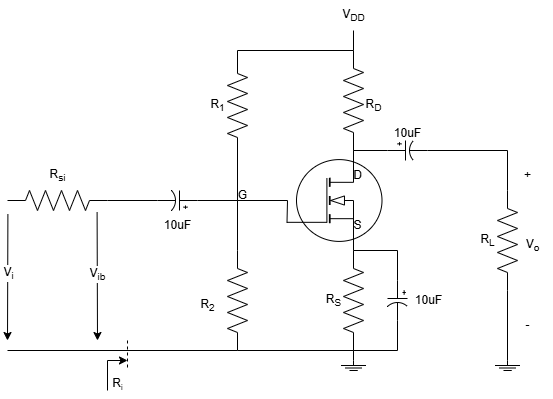
\includegraphics[width=0.65\linewidth]{Lab09/Lab9.drawio.png}
        \caption{Circuit Diagram}
        \label{l9f}
    \end{figure}
    \FloatBarrier

\section{Detailed Procedures}
    \subsection{Analyzation}


    \subsection{Procedures}

    
\section{Discussion}


\section{Conclusion}
